\chapter{MARCO CONCEPTUAL Y ESTADO DEL ARTE}

El presente capítulo expone los fundamentos conceptuales y el estado actual del conocimiento que sustentan el desarrollo del Desafío Bebras Bolivia. En primer lugar, se presentan las bases teóricas del pensamiento computacional como eje disciplinar central de la propuesta educativa de Bebras, así como sus componentes fundamentales y su relación con el diseño de tareas orientadas a estudiantes de nivel primario y secundario. Asimismo, se describe la organización internacional Bebras, su estructura, sus categorías de participación y los principios pedagógicos que orientan la construcción de ejercicios dentro del desafío.

Posteriormente, se desarrolla el estado del arte del Desafío Bebras a nivel internacional y regional, con énfasis en su alcance global, su presencia en América Latina y la situación actual de las plataformas tecnológicas empleadas por distintos países miembro. Esta revisión permite contextualizar académica y técnicamente el problema abordado en este trabajo, delimitar el alcance de la propuesta y justificar la necesidad de una plataforma propia adaptada al contexto boliviano.

\section{PENSAMIENTO COMPUTACIONAL}

El pensamiento computacional constituye el eje disciplinar del Desafío Bebras y, por tanto, el punto de partida obligatorio para comprender el propósito de la plataforma que se desarrolla en este trabajo. \textcite[33]{wing2006} lo define como el conjunto de procesos de pensamiento involucrados en la formulación de problemas y la representación de sus soluciones, de tal manera que un agente de procesamiento de información —humano o máquina— pueda ejecutarlas eficazmente. Esta definición es relevante porque desvincula el pensamiento computacional de la programación en sí misma: no se trata de enseñar a los estudiantes a operar una computadora, sino de desarrollar en ellos una forma de razonamiento sistemático aplicable a cualquier dominio del conocimiento.

\textcite[35]{wing2006} señala, además, que el pensamiento computacional comparte rasgos con el pensamiento matemático —en cuanto a la manera de abordar la resolución de problemas— y con el pensamiento de ingeniería —en cuanto al diseño y evaluación de sistemas complejos que interactúan con el mundo real—, pero se distingue de ambos por la naturaleza propia de la computación como disciplina. Esta característica interdisciplinaria explica por qué Bebras Internacional adoptó el pensamiento computacional como eje de sus competencias: las tareas propuestas no requieren conocimientos previos de programación, pero sí demandan la aplicación de estrategias cognitivas propias de las ciencias de la computación.

Desde una perspectiva educativa, \textcite[39]{grover2013} analizaron la evolución del concepto en el contexto escolar K--12 y concluyeron que, a pesar de la diversidad de interpretaciones surgidas a partir del trabajo seminal de Wing, existe consenso en identificar un conjunto de capacidades cognitivas centrales que definen el pensamiento computacional: la descomposición de problemas, el reconocimiento de patrones, la abstracción y el diseño de algoritmos. Estas cuatro capacidades son precisamente las que se ponen en juego en cada tarea del Desafío Bebras, y su comprensión es indispensable para el diseño del módulo de construcción de ejercicios contemplado en este proyecto.

\section{COMPONENTES DEL PENSAMIENTO COMPUTACIONAL}

Esta sección describe los cuatro componentes fundamentales del pensamiento computacional tal como son reconocidos en la literatura académica contemporánea. Cada uno de ellos tiene una correspondencia directa con las estrategias de resolución que los participantes del Desafío Bebras deben activar al enfrentarse a sus tareas, y con los criterios de diseño que los autores de ejercicios deben considerar al construir nuevos problemas dentro del sistema desarrollado en este trabajo.

\subsection{Descomposición}

La descomposición es el proceso cognitivo mediante el cual un problema complejo se divide en subproblemas más pequeños y manejables, cada uno de los cuales puede ser analizado y resuelto de manera independiente. \textcite[34]{wing2006} describe este proceso como una de las herramientas mentales esenciales del pensamiento computacional, señalando que es la base para abordar tareas de gran complejidad que ningún individuo podría resolver sin antes segmentarlas en partes más accesibles. En el contexto de una tarea Bebras, la descomposición se manifiesta cuando el estudiante identifica las partes constitutivas de un problema aparentemente difícil y trabaja sobre cada una de ellas antes de construir una solución integrada.

\subsection{Reconocimiento de patrones}

El reconocimiento de patrones consiste en identificar similitudes, regularidades o estructuras repetidas dentro de un problema o entre problemas distintos. \textcite[39]{grover2013} incluyen esta capacidad entre los componentes centrales del pensamiento computacional aplicado a la educación K--12, destacando su utilidad para transferir estrategias de solución ya conocidas a nuevos contextos. Desde el punto de vista del diseño de tareas, el reconocimiento de patrones es un componente que los autores de ejercicios deben calibrar con cuidado: si el patrón es demasiado evidente, la tarea pierde valor como instrumento de evaluación; si es demasiado oculto, puede resultar frustrante para el nivel académico al que está dirigida.

\subsection{Abstracción}

La abstracción implica identificar y conservar únicamente la información relevante de un problema, descartando los detalles que no contribuyen a su solución. \textcite[35]{wing2006} considera la abstracción como el concepto más poderoso de las ciencias de la computación, y afirma que el pensamiento a múltiples niveles de abstracción es la habilidad que distingue al pensador computacional de quien simplemente programa. En el contexto de Bebras, la abstracción aparece cuando el estudiante debe construir un modelo simplificado de una situación cotidiana para poder razonar sobre ella de manera eficiente. El módulo de construcción de ejercicios de este proyecto debe, por tanto, permitir a los autores especificar con precisión qué información es esencial para la tarea y cuál es meramente contextual.

\subsection{Diseño de algoritmos}

El diseño de algoritmos es el proceso de definir una secuencia finita y ordenada de pasos que conduce a la solución de un problema. \textcite[33]{wing2006} señala que formular un problema de manera que admita una solución algorítmica es en sí mismo un acto de pensamiento computacional, independientemente de si dicha solución será implementada por una persona o por una máquina. En las tareas Bebras, el diseño de algoritmos se evalúa de manera implícita cuando el estudiante debe determinar el orden correcto de una serie de acciones o construir una estrategia paso a paso para alcanzar un objetivo dentro del enunciado del problema.

La Figura~\ref{fig:componentes_pc} sintetiza los componentes del pensamiento computacional considerados en este trabajo y su relación con el diseño de tareas.

\begin{figure}[h]
    \centering
    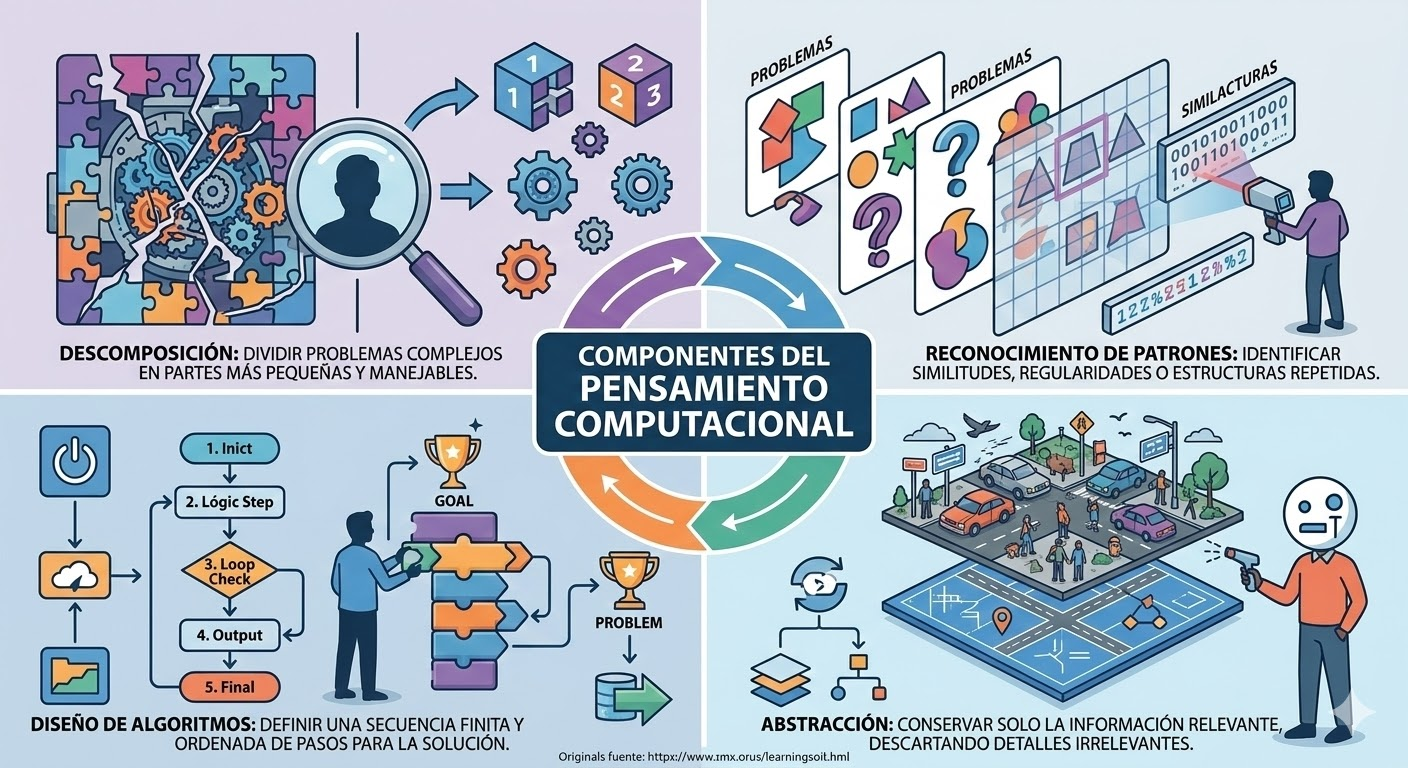
\includegraphics[width=0.7\textwidth]{assets/pensamiento_computacional.jpg}
    \caption[Componentes del Pensamiento Computacional]{Componentes del Pensamiento Computacional considerados en el diseño de tareas del Desafío Bebras - Elaboración propia}
    \label{fig:componentes_pc}
\end{figure}

\section{EL DESAFÍO BEBRAS INTERNACIONAL}

El Desafío Bebras constituye una de las iniciativas de informática y pensamiento computacional de mayor alcance internacional. \textcite{bebras} lo describe como el Desafío Internacional de Informática y Pensamiento Computacional, organizado anualmente con el propósito de acercar los conceptos fundamentales de la informática a estudiantes de nivel primario y secundario de todo el mundo. Para contextualizar la naturaleza y propósito de la organización sobre la cual se desarrolla la plataforma de este trabajo, es necesario comprender su origen, su modelo de participación y las características particulares del concurso que administra.

\subsection{Origen e historia de la organización}

\textcite{dagienefutschek2008} sitúan el origen del concurso en Lituania en 2004, impulsado por la profesora Valentina Dagienė. El nombre ``Bebras'' (castor, en lituano) alude al trabajo sistemático y la persistencia que el desafío busca fomentar en los estudiantes. Desde su primera edición nacional, la iniciativa se expandió de forma sostenida hasta consolidarse como una red internacional.

La Figura~\ref{fig:bebras2004} muestra una referencia visual de los primeros países participantes en los inicios de la organización.

\begin{figure}[htbp]
    \centering
    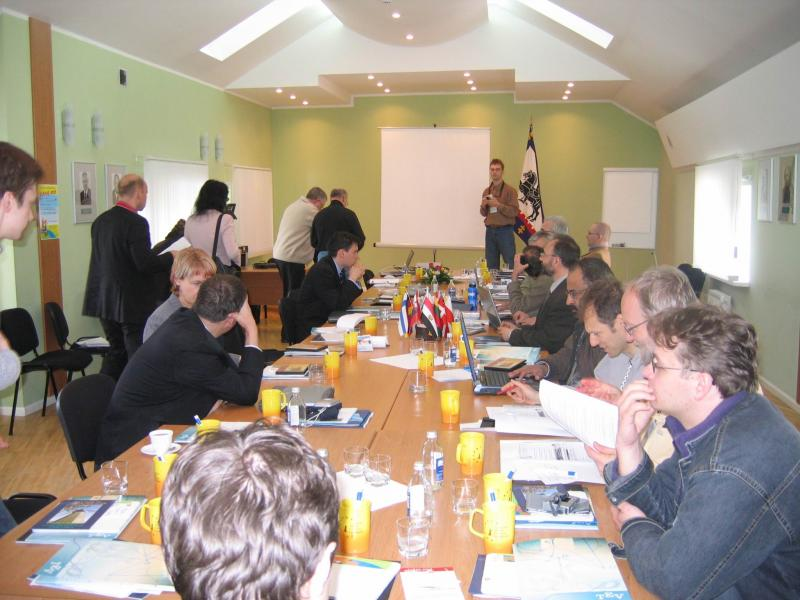
\includegraphics[width=0.65\textwidth]{assets/bebras2004.jpg}
    \caption[Primeros países de Bebras (2004)]{Primeros países vinculados al inicio de la organización Bebras en 2004. Galería oficial de Bebras \parencite{bebras}}
    \label{fig:bebras2004}
\end{figure}

De acuerdo con \textcite{bebras}, la organización reúne actualmente 96 países miembro y más de 2,5 millones de participantes anuales, siendo la competencia de ciencias de la computación de mayor alcance global. Este crecimiento se explica, en gran medida, por su enfoque inclusivo: no exige conocimientos previos de programación. Además, en 2015 recibió el ``Best Practices in Education Award'' de Informatics Europe, patrocinado por Microsoft \parencite{bebras}.

\subsection{Modelo de gobernanza y el \emph{Bebras Task Workshop}}

Un aspecto central del modelo internacional es el proceso mediante el cual se construye el banco de tareas que cada país utiliza en su edición nacional del concurso. \textcite{dagienefutschek2008} describen que las tareas no son creadas de manera centralizada por un único equipo, sino que son propuestas, revisadas y seleccionadas de manera colectiva por los representantes de todos los países miembro durante el denominado \emph{Bebras Task Workshop}, un taller internacional que se celebra anualmente. Este proceso colaborativo garantiza que las tareas reflejen una diversidad de contextos culturales y niveles de dificultad, y que sean validadas por expertos en informática educativa antes de ser incorporadas al banco oficial de problemas.

Este modelo de gobernanza es relevante para el presente proyecto porque implica que la plataforma de Bebras Bolivia debe ser capaz de incorporar y gestionar tareas provenientes del banco internacional, adaptando sus enunciados y contextos al entorno educativo boliviano cuando sea pertinente.

\section{ESTRUCTURA DEL DESAFÍO BEBRAS}

La estructura formal del Desafío Bebras está estandarizada a nivel internacional, aunque cada país miembro tiene la potestad de adaptar ciertos elementos —como los nombres de las categorías de edad o el calendario de realización— a su propio contexto educativo. A continuación, se describen los elementos estructurales fundamentales del concurso tal como son definidos por la organización internacional y adoptados con variaciones por las iniciativas nacionales analizadas durante el desarrollo de este proyecto.

\subsection{Categorías de participación}

\textcite{bebraseeuu} organiza el desafío en seis categorías etarias, cada una con tareas ajustadas al nivel cognitivo esperado: Kits (6--8), Castors (8--10), Benjamins (10--12), Cadets (12--14), Juniors (14--16) y Seniors (16--18). Esta segmentación busca mantener coherencia entre dificultad, temática y edad de los participantes.

Como adaptación nacional, \textcite{bebrasperu} emplea categorías con denominaciones culturales propias (Caral, Kuélap, Machu Picchu y Chan Chan), conservando la lógica de progresión por edad. Este antecedente confirma que el modelo Bebras permite contextualización local sin afectar la comparabilidad internacional de resultados.

\subsection{Formato y duración del concurso}

\textcite{dagienefutschek2008} describen que cada participante dispone de 45 minutos para resolver un conjunto de tareas de opción múltiple e interactivas, agrupadas en tres niveles de dificultad: fácil, medio y difícil. \textcite{bebras} especifica que el conjunto estándar comprende 15 tareas distribuidas en tres bloques de cinco, aunque para las categorías de menor edad este número se reduce a bloques de tres y cuatro tareas respectivamente, en consideración a las capacidades cognitivas del grupo. En la gran mayoría de los países participantes, el concurso se realiza en línea a través de un sistema web que califica automáticamente las respuestas de cada participante al finalizar el tiempo establecido.

\subsection{Tipos de tareas}

\textcite{dagienefutschek2008} identifican dos tipos generales de problemas utilizados en el concurso: las tareas de opción múltiple y las tareas interactivas. Ambas comparten características comunes que constituyen los criterios de calidad del banco de problemas: son breves, respondibles en pocos minutos, no requieren conocimientos previos de programación, están claramente vinculadas a conceptos fundamentales de la informática y deben resultar atractivas y motivadoras para el rango de edad al que están dirigidas. La dimensión interactiva de algunas tareas —donde el estudiante manipula elementos en pantalla en lugar de simplemente seleccionar una respuesta— añade un componente de exploración que se alinea con los principios del aprendizaje activo.

\section{CRITERIOS PARA EL DISEÑO DE TAREAS BEBRAS}

El módulo de construcción de ejercicios de pensamiento computacional constituye el componente de mayor complejidad funcional dentro del sistema desarrollado en este trabajo. A diferencia de la \textit{landing page} o del módulo de inscripciones, cuyo alcance está delimitado por flujos de usuario relativamente convencionales, el módulo de creación de tareas debe contemplar restricciones pedagógicas específicas que determinan qué constituye un ejercicio válido dentro del estándar internacional Bebras. Por esta razón, es indispensable comprender los criterios que la comunidad académica y el comité internacional han establecido para la evaluación y selección de tareas, ya que estos criterios definen directamente los campos, validaciones y capacidades que el sistema debe ofrecer a los autores de ejercicios.

\subsection{Criterios pedagógicos fundamentales}

\textcite{dagienefutschek2008} identifican los criterios centrales que debe cumplir una tarea del Desafío Bebras para ser considerada de calidad. En primer lugar, la tarea debe estar vinculada de manera clara y demostrable a uno o más conceptos fundamentales de la informática, de modo que su resolución no sea trivialmente reducible a conocimiento general o habilidades matemáticas básicas. En segundo lugar, debe ser respondible en pocos minutos sin requerir conocimientos previos de programación ni preparación específica, condición que garantiza la equidad entre participantes de distinto perfil educativo. En tercer lugar, el enunciado debe resultar atractivo y motivador para el rango de edad al que está dirigida, lo que implica que la situación planteada sea reconocible y relevante para la experiencia cotidiana del estudiante. Por último, la solución debe ser verificable de manera objetiva, ya sea mediante opción múltiple o mediante una interacción que produce un resultado unívoco, lo cual es indispensable para la corrección automática que caracteriza al sistema de evaluación en línea de Bebras. Este ciclo de diseño se resume en la Figura~\ref{fig:ciclo_bebras}.

\begin{figure}[h]
    \centering
    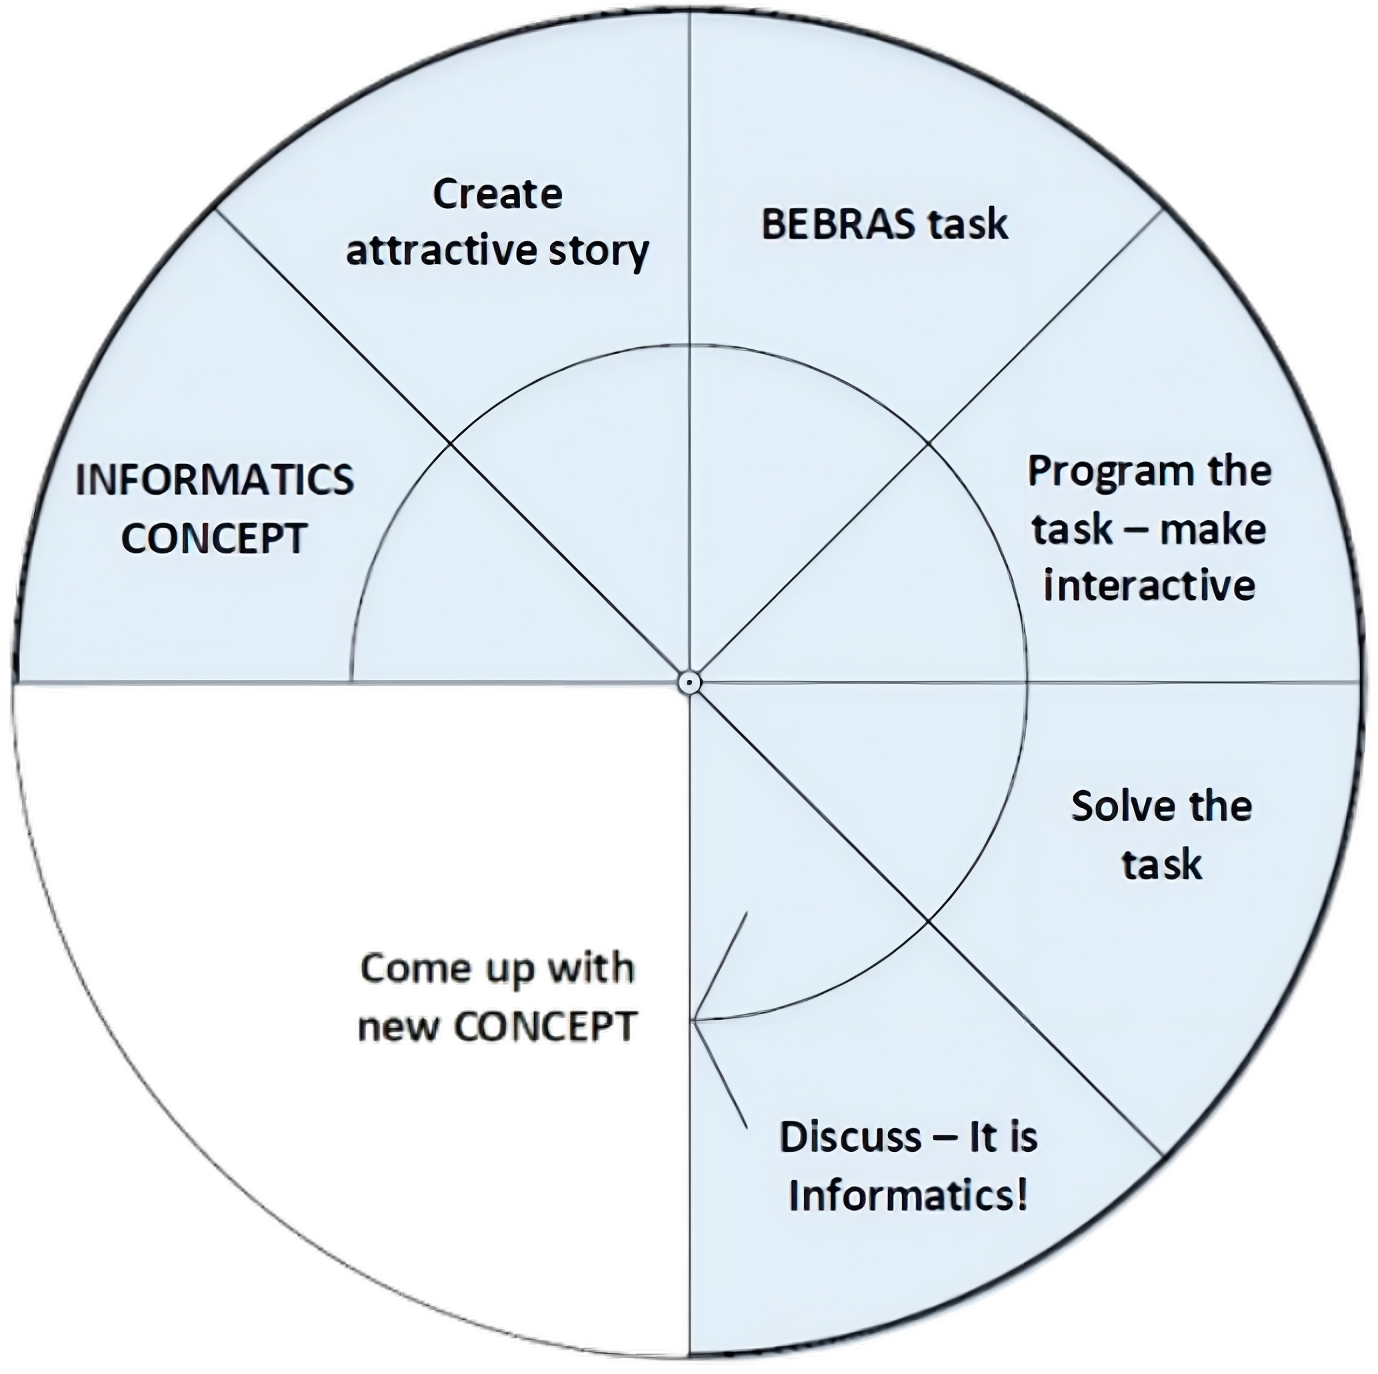
\includegraphics[width=0.5\textwidth]{assets/fig_dagiene2008.png}
    \caption[Ciclo de diseño de una tarea Bebras]{Ciclo de diseño de una tarea Bebras desde el concepto de informática hasta la comprensión del estudiante \parencite[p.~25]{dagienefutschek2008}}
    \label{fig:ciclo_bebras}
\end{figure}

\subsection{Tipos de tareas: opción múltiple e interactivas}

\textcite{dagienefutschek2008} distinguen dos tipos generales de problemas dentro del catálogo Bebras. Las tareas de opción múltiple presentan un enunciado acompañado de un conjunto cerrado de alternativas de respuesta, de las cuales únicamente una es correcta; su ventaja principal es la simplicidad de implementación y corrección automática. Las tareas interactivas, por su parte, incorporan un elemento manipulable en pantalla —como un grafo, una cuadrícula, una secuencia de elementos o un diagrama— que el participante debe modificar o completar para producir una solución; este formato añade una dimensión de exploración activa que favorece la comprensión de conceptos dinámicos como ordenamiento, recorrido de estructuras o simulación de procesos. En la Figura~\ref{fig:tipos_tareas} se ilustran ejemplos reales de ambos formatos.

\begin{figure}[h]
    \centering
    \begin{subfigure}[b]{0.65\textwidth}
        \centering
        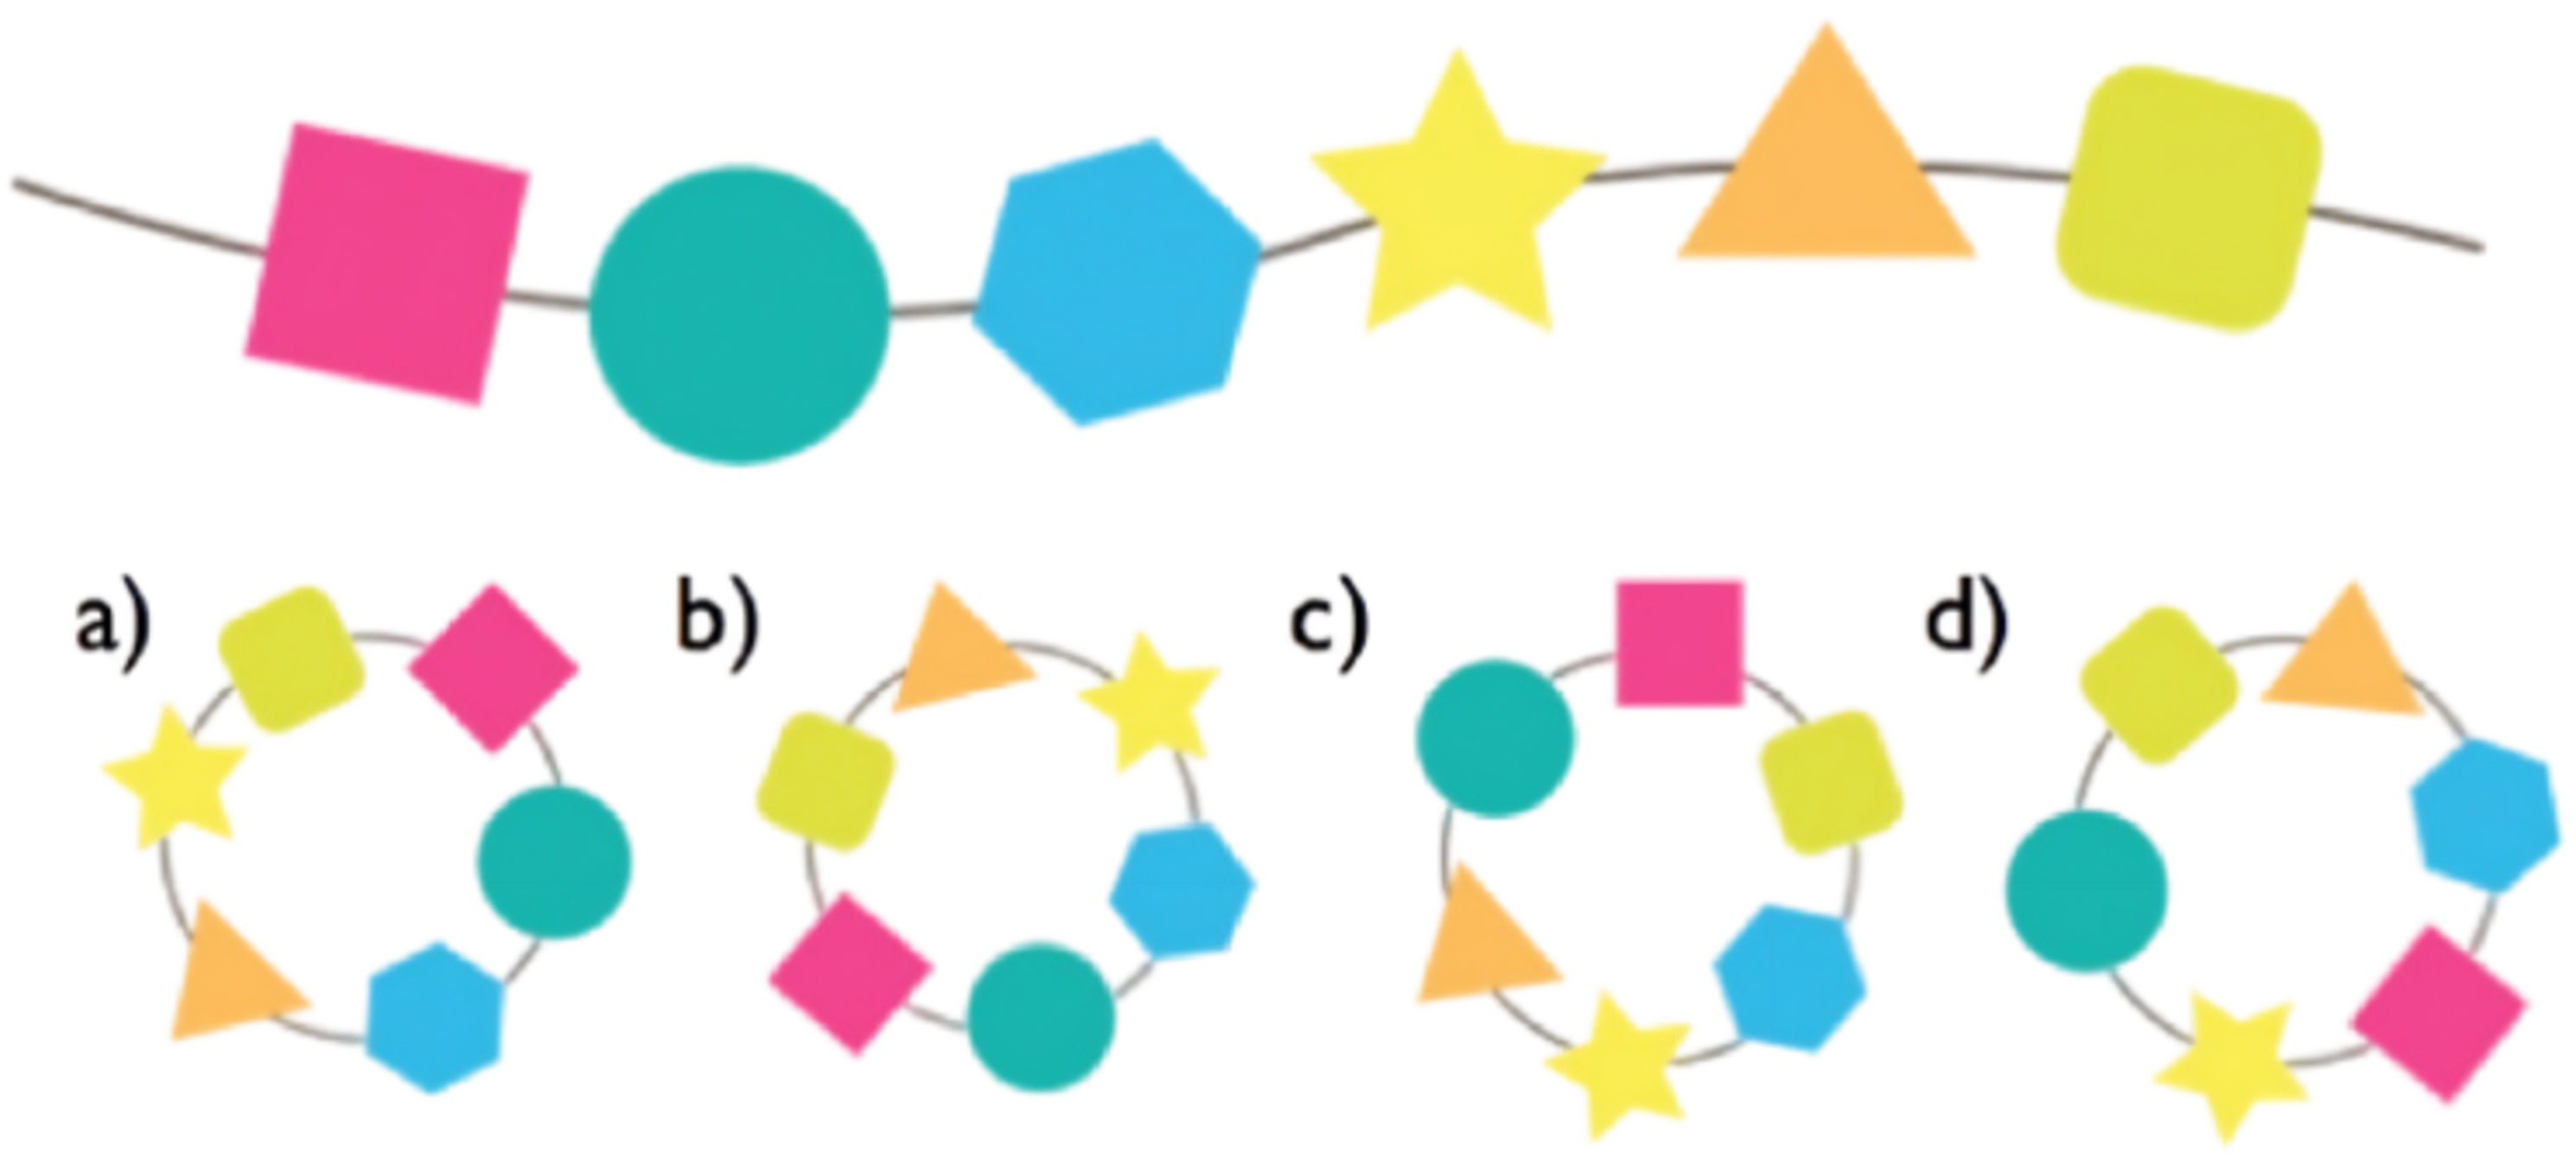
\includegraphics[width=\textwidth]{assets/fig_tarea_opcion.png}
        \caption{Tarea de opción múltiple (Task 2015-MY-01)}
        \label{fig:tarea_opcion}
    \end{subfigure}

    \vspace{0.5cm}

    \begin{subfigure}[b]{0.65\textwidth}
        \centering
        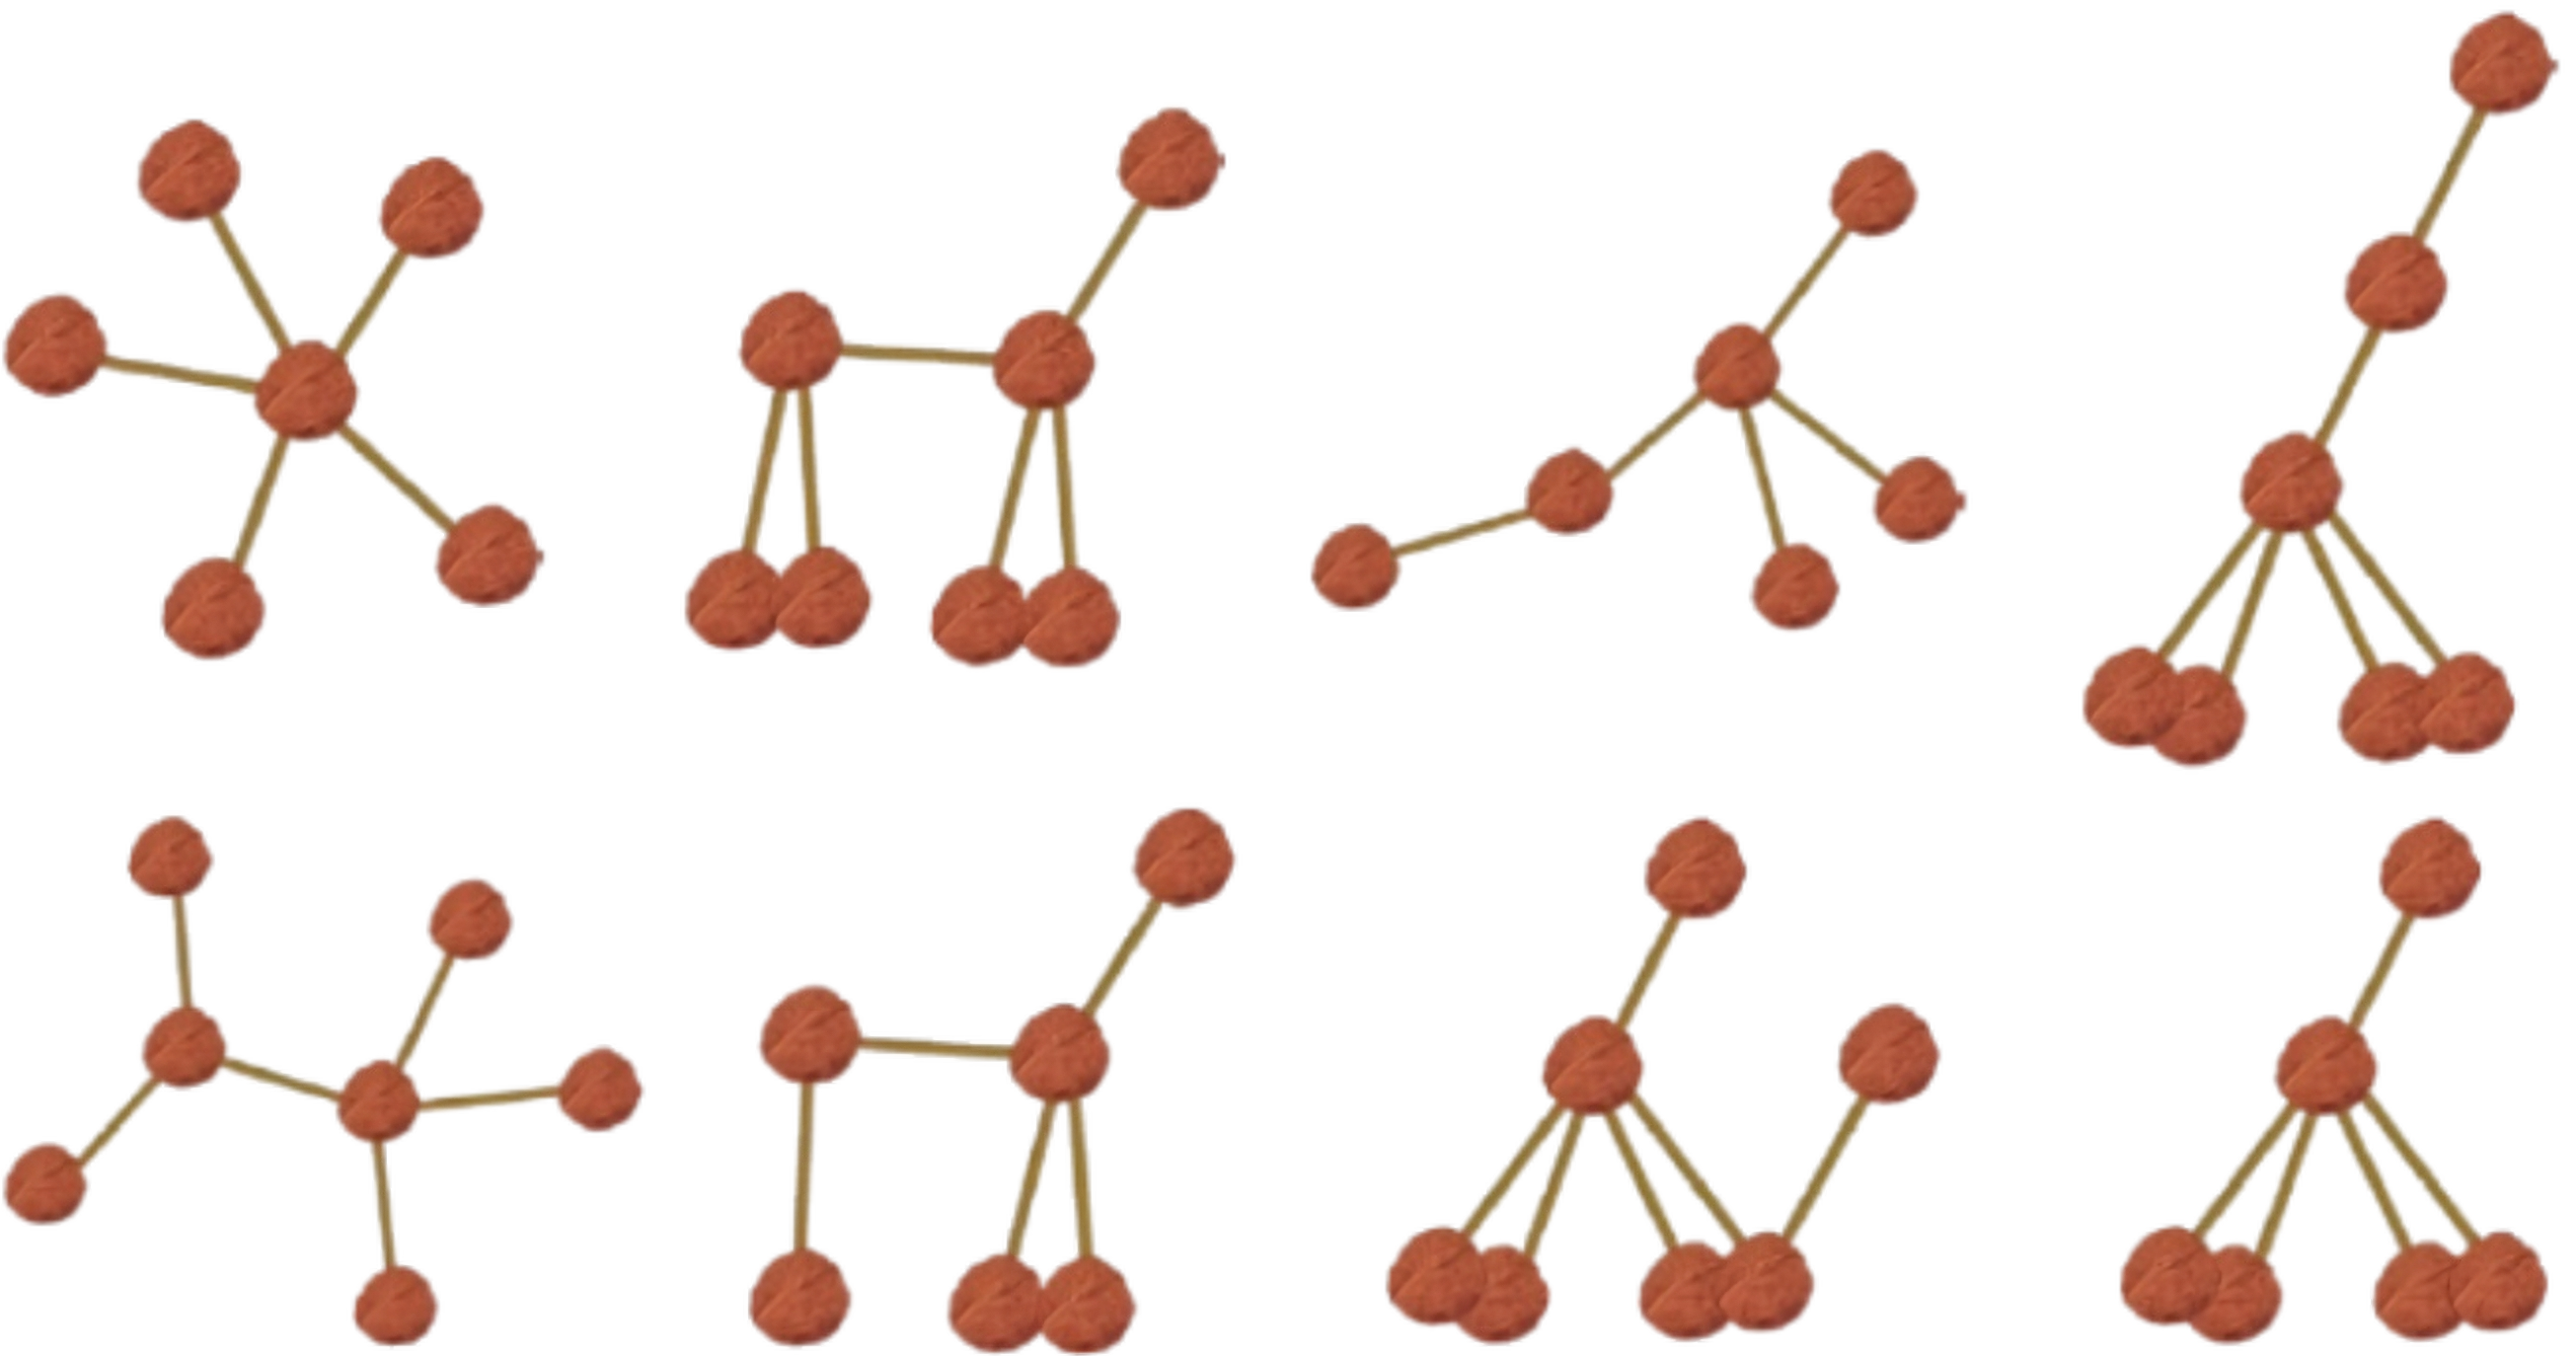
\includegraphics[width=\textwidth]{assets/fig_tarea_interactiva.png}
        \caption{Tarea interactiva (Task 2015-CZ-01)}
        \label{fig:tarea_interactiva}
    \end{subfigure}

    \caption[Ejemplos de tareas del Desafío Bebras]{Ejemplos de tareas del Desafío Bebras: opción múltiple e interactiva \parencite[pp.~41--43]{izumirolo2017}}
    \label{fig:tipos_tareas}
\end{figure}

\subsection{Niveles de dificultad y adecuación al nivel académico}

\textcite{dagienestupuriene2016} señalan que la asignación de una tarea a un nivel de dificultad —fácil, medio o difícil— dentro de una categoría de edad no es arbitraria, sino que responde a criterios relacionados con la carga cognitiva que la tarea impone al participante: el número de pasos necesarios para llegar a la solución, el grado de abstracción requerido, la cantidad de información irrelevante presente en el enunciado y la familiaridad del contexto narrativo para el grupo de edad. Esta calibración es responsabilidad de los autores de tareas y del comité de revisión, y constituye uno de los aspectos más críticos del proceso de validación que precede a la incorporación de un ejercicio al banco oficial.

Para la plataforma de Bebras Bolivia, este criterio implica que el módulo de construcción de ejercicios debe incluir un flujo de revisión y aprobación que permita al comité evaluador validar la idoneidad pedagógica de cada tarea antes de que esta quede disponible para ser asignada a un examen. La implementación de este flujo de trabajo es una de las capacidades documentadas en el análisis de requisitos del sistema.

\section{ESTADO DEL ARTE}

El estado del arte de este trabajo examina la situación actual del Desafío Bebras desde una perspectiva internacional, regional y tecnológica. Esta revisión permite identificar el nivel de consolidación alcanzado por la iniciativa a escala global, reconocer su presencia todavía emergente en América Latina y analizar las plataformas tecnológicas desarrolladas por distintos países miembro. En conjunto, estos antecedentes justifican la pertinencia de proponer una solución propia para Bebras Bolivia.

\subsection{Alcance global del Desafío Bebras}

Desde su primera edición en Lituania en 2004, el Desafío Bebras ha experimentado un crecimiento sostenido que lo ha consolidado como la competencia de ciencias de la computación de mayor alcance en el mundo. \textcite{bebras} reporta que la organización cuenta actualmente con 96 países miembro y supera los 2,5 millones de participantes anuales. La dimensión de esta expansión puede apreciarse también en la escala de participación de países específicos: Francia registra alrededor de 700.000 participantes al año, Alemania cerca de 500.000 y el Reino Unido aproximadamente 400.000, según datos publicados por organizaciones nacionales miembro de la red Bebras \parencite{bebraseeuu}.

\textcite{izumirolo2017} realizaron el primer estudio multinacional de gran escala sobre el desempeño en tareas Bebras, analizando datos de rendimiento de 115.400 estudiantes de grados 3 a 12 en siete países. Sus resultados confirmaron que las tareas de algoritmos y representación de datos concentran entre el 75 y el 90 por ciento del banco de problemas, mientras que categorías como abstracción, paralelización y descomposición de problemas tienen una presencia menor pero significativa en los distintos grupos de edad. Este estudio estableció las bases metodológicas para el uso de las tareas Bebras como instrumento de evaluación del pensamiento computacional más allá del contexto competitivo, validando su pertinencia para entornos curriculares formales.

\begin{figure}[h]
    \centering
    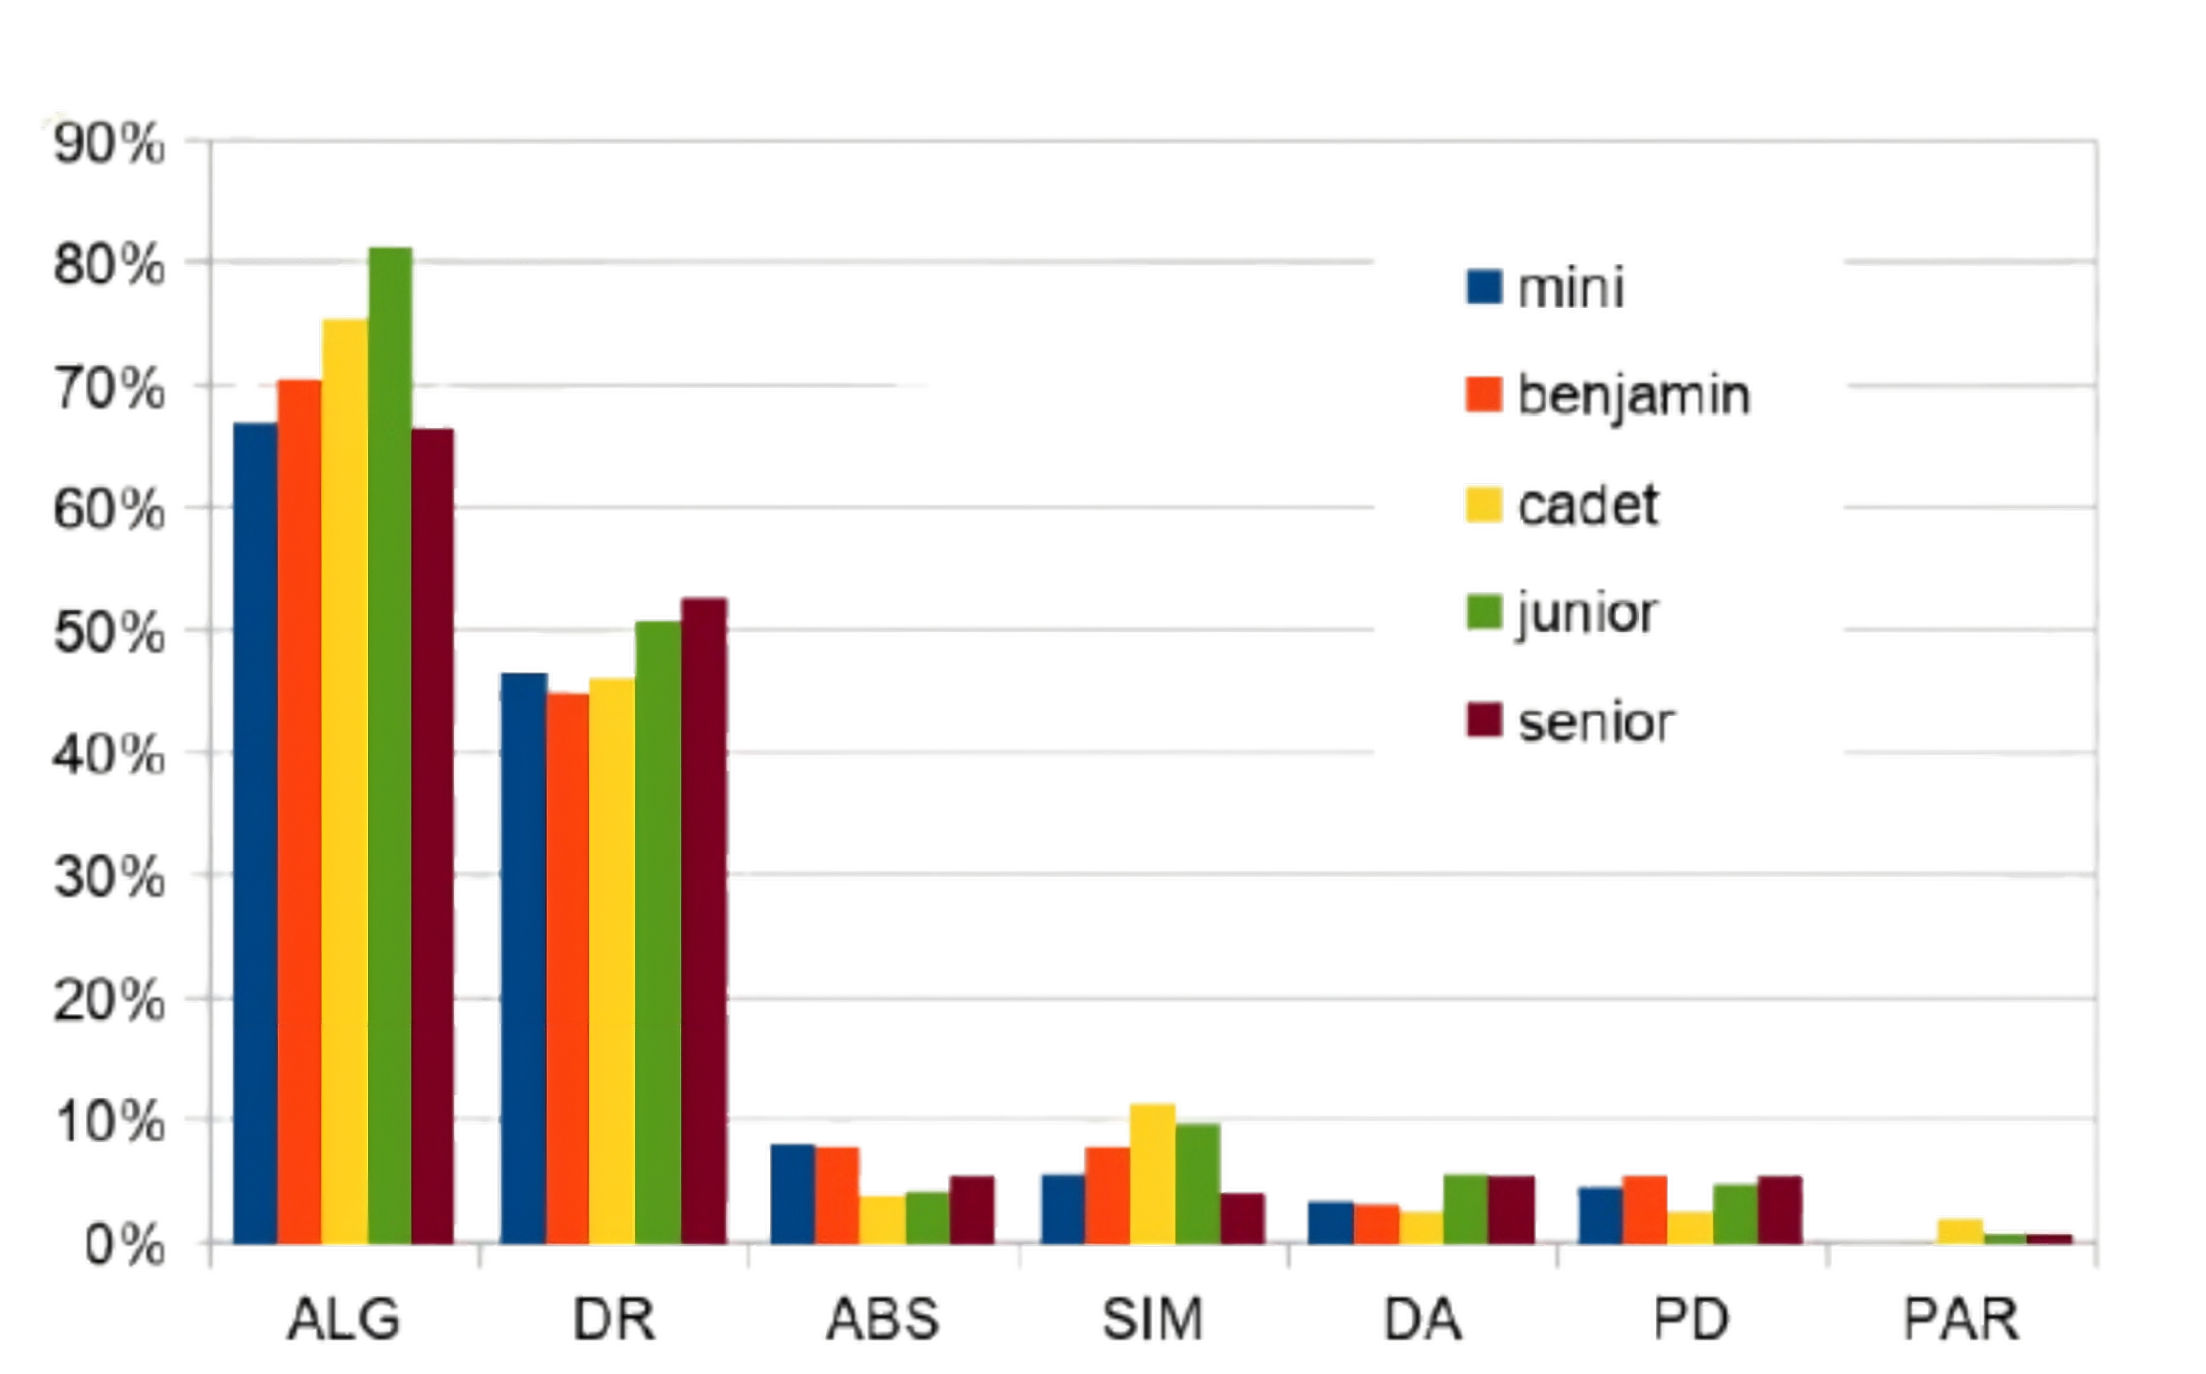
\includegraphics[width=0.6\textwidth]{assets/bebras_challenge_statistics.png}
    \caption[Distribución de categorías de pensamiento computacional en tareas Bebras]{Distribución de categorías de pensamiento computacional en tareas Bebras por grupo de edad \parencite[p.~47]{izumirolo2017}}
    \label{fig:categorias_bebras}
\end{figure}

\subsection{Bebras en América Latina}

La presencia de Bebras en América Latina es todavía incipiente en comparación con Europa y Asia. Entre los países de la región con mayor trayectoria se encuentra Uruguay, cuyo programa nacional de pensamiento computacional integra las tareas Bebras en el currículo escolar desde 2017 y ha alcanzado a más de 70.000 estudiantes \parencite{olmo2024}. \textcite{bavera2024} validaron en una universidad latinoamericana un instrumento de evaluación del pensamiento computacional construido a partir de tareas Bebras traducidas al español, aplicado a una muestra de 980 estudiantes de primer año sin experiencia previa en programación, obteniendo correlaciones positivas y significativas con otras métricas académicas establecidas. Este antecedente es pertinente porque demuestra la viabilidad de adaptar el modelo Bebras al contexto educativo hispanohablante sin pérdida de rigor conceptual.

En el caso específico de Bolivia, el Desafío Bebras no cuenta con una edición nacional establecida ni con una plataforma tecnológica propia que permita su administración en línea. La participación de estudiantes bolivianos en el concurso ha sido hasta ahora esporádica y sin la infraestructura institucional que caracteriza a los países miembro activos de la organización internacional. Esta situación configura el problema central que motiva el presente proyecto: la ausencia de un sistema propio adaptado al contexto boliviano impide la consolidación de Bebras Bolivia como una iniciativa educativa sostenible y comparable con las de otros países de la región.

\subsection{Estado de las plataformas tecnológicas Bebras}

No existe un sistema centralizado único que todos los países miembro de Bebras estén obligados a utilizar. \textcite{dagienefutschek2008} observaron que, desde los primeros años del concurso, cada país desarrolló o adoptó su propia infraestructura tecnológica para administrar el desafío, lo que ha resultado en una diversidad considerable de soluciones técnicas a nivel mundial. Esta descentralización es una característica deliberada del modelo de gobernanza de Bebras: garantiza la autonomía de cada país para adaptar el sistema a sus necesidades locales, pero implica también que no existe una plataforma de referencia única que pueda ser adoptada directamente.

El análisis de plataformas internacionales muestra que existen implementaciones maduras y funcionales, aunque desarrolladas con prioridades y arquitecturas distintas. Algunas privilegian la administración integral del concurso, mientras que otras enfatizan la difusión pública, la práctica libre o la gestión de contenido institucional. En consecuencia, el desarrollo de una plataforma propia para Bebras Bolivia no responde a la inexistencia total de antecedentes, sino a la necesidad de integrar en una sola solución capacidades que actualmente aparecen dispersas en diferentes implementaciones nacionales.